\documentclass[conference]{IEEEtran}

\usepackage[T1]{fontenc}
\usepackage[spanish,es-nodecimaldot,es-noshorthands]{babel}

\usepackage{subcaption}
\usepackage{graphicx}
\usepackage{amsmath}
\usepackage{tikz}
\usetikzlibrary{arrows.meta, positioning, fit, backgrounds, shapes.geometric, babel}
\usepackage{float}
\usepackage[colorlinks=true, linkcolor=black, citecolor=black, urlcolor=blue]{hyperref}
\usepackage{dblfloatfix}
\usepackage{placeins}

\hyphenation{op-tical net-works semi-conduc-tor}

\begin{document}

\title{Clasificación Automática Multiclase de Estadios del Sueño mediante Inteligencia Artificial y Señales Polisomnográficas Multimodales}

\author{
\IEEEauthorblockN{
    Juan David Rozo Verástegui,
    Jhoan Sebastián Saavedra Romero\\
    Juan Javier Valera Mejías,
    Juan Carlos Gamboa Peñaranda
}
\IEEEauthorblockA{
    Maestría en Inteligencia Artificial\\
    Universidad de los Andes\\
    Bogotá, Colombia
}
}

\maketitle

\begin{abstract}
La estadificación automática del sueño exige distinguir etapas breves como N1 y generalizar entre equipos de registro. En \textit{Sleep-EDF Expanded} comparamos dos formas de combinar señales polisomnográficas. En V4--V7, LightGBM clasifica representaciones de una red convolucional recurrente (CRNN), enriquecidas en V7 con descriptores espectrales nocturnos. En el experimento 8 (V8), un LightGBM con descarte de árboles (DART) y una CRNN espectral aprenden por separado y combinan sus probabilidades por estadio. La comparación principal se realizó sobre las mismas 20 noches de 10 sujetos de \textit{Sleep-Cassette}, con $24\,101$ épocas de 30 s y un margen de vigilia de 30 min. En V7, el perfil sin suavizado obtuvo 0.7286 de F1 macro y 0.4144 de F1 en N1. Al aplicar un modelo oculto de Markov (HMM), la exactitud subió a 0.7993 y el F1 en N1 bajó a 0.3933. Reentrenada con las 84 noches de desarrollo, la fusión V8 (59\,\% DART, 41\,\% CRNN) alcanzó 0.7791 de F1 macro, 0.8311 de exactitud, 0.7699 de kappa y 0.4959 de F1 en N1. La ganancia sobre DART solo fue pequeña y su intervalo pareado incluyó cero.
\end{abstract}

\begin{IEEEkeywords}
Clasificación de estadios del sueño, polisomnografía, redes neuronales convolucionales recurrentes, LightGBM, DART, fusión de probabilidades, Modelos Ocultos de Markov, generalización multicohorte.
\end{IEEEkeywords}

\IEEEpeerreviewmaketitle

%===========================================================
\section{Introducción}
%===========================================================
El sueño es una función fisiológica esencial; su alteración crónica está directamente asociada con el desarrollo de patologías cardiovasculares, neurológicas, respiratorias y metabólicas. El estándar de oro para su diagnóstico clínico es la polisomnografía (PSG), que registra de forma continua bioseñales multimodales como la electroencefalografía (EEG), la electrooculografía (EOG) y la electromiografía (EMG). Un componente obligatorio de este análisis es la estadificación del sueño (\textit{sleep staging}), donde cada segmento de 30 segundos (época) se clasifica en uno de los cinco estadios definidos por la Academia Americana de Medicina del Sueño (AASM): Vigilia (W), N1, N2, N3 y REM \cite{berry2020}.

En la práctica clínica actual, la estadificación es estrictamente manual y exige revisar visualmente entre 800 y 1,200 épocas por paciente. Esto genera un cuello de botella operativo y financiero que retrasa la entrega de resultados. Además, las fases de transición como N1 presentan una elevada variabilidad inter-evaluador debido a su naturaleza breve y ambigua \cite{berry2020}, reflejando la complejidad de la microcontinuidad neuronal subyacente \cite{kemp2000}.

Desde la Inteligencia Artificial (IA), automatizar este proceso enfrenta dos retos principales: un severo desbalance clínico de clases y la heterogeneidad entre pacientes y equipos de registro (\textit{Domain Shift}). Aunque diversas arquitecturas alcanzan exactitudes prometedoras con canales aislados \cite{supratak2020}, suelen subutilizar la información multimodal y degradar su rendimiento fuera de su cohorte de origen.

Estudiamos dos preguntas. Primero, ¿cuánto aporta a una CRNN multimodal la incorporación de información espectral y contexto nocturno en el clasificador tabular? Segundo, si ambas ramas conservan su propia decisión por estadio, ¿mejora la combinación respecto de cada rama y del mejor perfil anterior? La primera pregunta guía las fases V4--V7. La segunda retoma la exploración tabular de V2 y motiva el experimento 8. Comparamos las predicciones de época con el hipnograma de referencia, con especial atención a N1.

%===========================================================
\section{Estado del Arte y Revisión Bibliográfica}
%===========================================================
El análisis automático de estadios del sueño ha evolucionado rápidamente. Los enfoques iniciales dependían de la extracción manual de características en tiempo y frecuencia acopladas a modelos clásicos como Máquinas de Vectores de Soporte (SVM) y Bosques Aleatorios, limitados por heurísticas rígidas.

Con el aprendizaje profundo (\textit{Deep Learning}), arquitecturas seminales como DeepSleepNet \cite{supratak2017} combinaron Redes Neuronales Convolucionales (CNN) unidimensionales con capas recurrentes (LSTM) directamente sobre señales crudas. Trabajos posteriores como U-Sleep \cite{perslev2021} y L-SeqSleepNet \cite{phan2023} escalaron el modelado a ciclos completos de sueño, mientras que propuestas como AttnSleep \cite{eldele2021} incorporaron mecanismos de atención para capturar dependencias temporales.

No obstante, un obstáculo persistente en el aprendizaje profundo es el desplazamiento de dominio (\textit{Domain Shift}). Como fenómeno general documentado en redes neuronales profundas, los modelos pueden recurrir a atajos predictivos (\textit{Shortcut Learning}) basados en correlaciones espurias del conjunto de entrenamiento en lugar de características generalizables \cite{geirhos2020shortcut}. En polisomnografía, esto se traduce en caídas de rendimiento al evaluar redes entrenadas en una única cohorte sobre poblaciones o equipos de registro distintos. Por ello, resulta fundamental emplear señales polisomnográficas directas (EEG, EOG y EMG) en lugar de aproximaciones periféricas como la fotopletismografía (PPG).

Desde la perspectiva neurofisiológica de la AASM \cite{berry2020}, cada estadio exhibe firmas espectrales distintivas: la Vigilia (W) presenta ritmo Alfa (8--12 Hz) y tono muscular elevado; N1 se define por la atenuación del ritmo Alfa en más del 50\% de la época y la aparición de ondas Theta (4--8 Hz) en microeventos de 10 a 15 segundos; N2 consolida husos de sueño (12--16 Hz) y complejos K; N3 muestra ondas lentas Delta (0.3--4 Hz) de alta amplitud; y REM combina actividad EEG mixta de bajo voltaje con movimientos oculares rápidos (EOG) y atonía muscular (EMG). Sin embargo, las CNN con promediado global (\textit{Global Average Pooling}) sobre 30 segundos tienden a diluir los microeventos breves de N1, y la normalización estrictamente local por época elimina la referencia de energía basal nocturna del paciente.

En este contexto, hibridar extractores profundos con motores tabulares enriquecidos espectralmente y post-procesamiento probabilístico mediante Modelos Ocultos de Markov (HMM) constituye una alternativa robusta para el modelado secuencial del sueño.

%===========================================================
\section{Metodología}
%===========================================================
La concepción metodológica se estructuró mediante un estudio de ablación progresivo. Cada iteración buscó resolver una limitación empírica de la fase anterior frente a la heterogeneidad biológica y técnica de los registros.

\subsection{Datos y Preprocesamiento de Señales}
El estudio se basó en la base de datos pública \textit{Sleep-EDF Database Expanded} \cite{sleepedfx_dataset}, \cite{goldberger2000}, fusionando dos cohortes:
\begin{itemize}
    \item \textbf{Cohorte Clínica (\textit{Sleep-Telemetry}):} 44 noches de 22 sujetos con trastornos del sueño leves.
    \item \textbf{Cohorte Externa (\textit{Sleep-Cassette}):} Las primeras 40 noches (21 sujetos únicos) se integraron al entrenamiento multicohorte. Para conformar el conjunto de validación externa fijo (\textit{Hold-Out}), se seleccionaron las siguientes 20 noches estrictamente disjuntas por sujeto (10 sujetos únicos, $24\,101$ épocas), excluyendo cualquier registro perteneciente a sujetos presentes en entrenamiento.
\end{itemize}

En las 44 noches de \textit{Telemetry}, antes del recorte de vigilia, N2 domina la distribución ($\approx$46.5\%), mientras que N1 representa una minoría crítica (8.6\%). El F1 macro es la media de los cinco F1 por estadio y otorga a N1 el mismo peso que a N2. También se informa la exactitud por época y el kappa de Cohen, que ajusta la concordancia por la esperada al azar.

Para comparar V4--V8 en la reserva fija y limitar el peso de la vigilia diurna de \textit{Sleep-Cassette}, se seleccionaron las épocas puntuables conservando un margen estricto de $\pm$30 minutos antes del primer y después del último episodio de sueño (N1, N2, N3 o REM). El \textit{pipeline} de V4--V7 procesa cuatro canales (EEG Fpz-Cz, EEG Pz-Oz, EOG horizontal y EMG submental) mediante MNE-Python \cite{gramfort2013} (ver Figura \ref{fig:pipeline_stateless}). Dado que \textit{Sleep-Cassette} almacena la EMG submental como envolvente a baja frecuencia (1 Hz), la lectura con MNE remuestrea automáticamente todos los canales a 100 Hz ($3\,000$ muestras por época). Se aplicó un filtro FIR pasabanda de fase cero (0.3--35.0 Hz) para preservar la morfología de los microeventos EEG \cite{berry2020}; se reconoce que este corte atenúa frecuencias altas de la EMG, limitando su rol a un indicador auxiliar de tono basal. Para garantizar continuidad operativa ante la ausencia física de canales auxiliares (siempre que exista al menos un canal EEG), el \textit{pipeline} implementa \textit{Zero Imputation} inyectando tensores nulos. Finalmente, la amplitud se estandarizó con Z-Score local por época para la rama profunda, complementada en V7 con normalización espectral nocturna.

\begin{figure}[htbp]
\centering
\begin{tikzpicture}[
 font=\footnotesize, node distance=3mm and 4mm,
 paso/.style={draw, rounded corners, align=center, inner sep=3pt, text width=.40\columnwidth},
 flecha/.style={-{Stealth[length=1.7mm]}, semithick}]
\node[paso, fill=green!8] (psg) {Lectura de señales\\disponibles en el EDF};
\node[paso, right=of psg] (filtro) {Filtro FIR\\0.3--35 Hz};
\node[paso, below=of filtro] (tensor) {Épocas de 30 s\\canal ausente a cero};
\node[paso, left=of tensor] (norma) {Z-score local\\por época y canal};
\draw[flecha] (psg) -- (filtro);
\draw[flecha] (filtro) -- (tensor);
\draw[flecha] (tensor) -- (norma);
\end{tikzpicture}
\caption{Preparación de la entrada de señal para las CRNN de V4--V7.}
\label{fig:pipeline_stateless}
\end{figure}

\subsection{Diseño Experimental y Entorno de Reproducibilidad}
Durante la fase exploratoria sobre la cohorte clínica (V4), se utilizó validación cruzada \textit{Leave-One-Subject-Out} (LOSO). Al escalar al entrenamiento multicohorte (V5--V7, 84 noches) con \textit{Data Augmentation} en memoria, LOSO resultó computacionalmente inviable y se transicionó a \textit{GroupKFold} de 5 pliegues agrupado por identificador único de sujeto (prefijos \texttt{ST\_} y \texttt{SC\_}).

Los entrenamientos de las CRNN de V4--V7 se ejecutaron en Google Colab sobre GPU NVIDIA A100. La CRNN (246,053 parámetros) procesó secuencias de 15 épocas (\texttt{SEQ\_LEN=15}) con tamaño de lote de 128 (\texttt{BATCH\_SIZE=128}). La selección de hiperparámetros tabulares se realizó con Optuna (TPE) \cite{akiba2019optuna} y la calibración de pesos de clase en V7 empleó \textit{GroupShuffleSplit} (20\% validación interna, semilla 42).

\subsection{Evolución Arquitectónica (Estudio de Ablación)}
En la reserva inicial de \textit{Telemetry} (5 sujetos, $9\,929$ épocas), Random Forest alcanzó 0.7320 de F1 macro y LightGBM alcanzó 0.7541 sobre las mismas observaciones. Este resultado motivó explorar descriptores temporales y espectrales en V2. En paralelo, V3 ensayó convoluciones separadas para EEG, EOG y EMG antes de una BiLSTM para aprender la sucesión de estadios. Esta línea produjo la representación latente de V4 (Figura~\ref{fig:arq_v4}). El experimento 8 retoma la línea tabular y la combina con una red que aprende sobre el espectro nocturno.

% --- FIGURA COMPARATIVA V4 vs V7 ---
\begin{figure*}[htbp]
\centering

% --- MINIPAGE 1: MODELO V4 ---
\begin{minipage}{0.48\textwidth}
\centering
\resizebox{\linewidth}{!}{%
\begin{tikzpicture}[
    >=Latex,
    node distance=0.6cm and 0.5cm,
    font=\sffamily\small,
    input/.style={draw, rectangle, rounded corners, fill=blue!10, minimum width=2.5cm, minimum height=0.8cm, align=center},
    cnn/.style={draw, rectangle, fill=orange!15, minimum width=3cm, minimum height=1.5cm, align=center},
    fusion/.style={draw, rectangle, fill=gray!20, minimum width=5cm, minimum height=0.8cm, align=center},
    attention/.style={draw, ellipse, fill=yellow!20, minimum width=3cm, minimum height=0.8cm, align=center},
    lstm/.style={draw, rectangle, rounded corners, fill=green!15, minimum width=4cm, minimum height=0.8cm, align=center},
    dense/.style={draw, rectangle, fill=purple!15, minimum width=4cm, minimum height=0.8cm, align=center},
    lgbm/.style={draw, rectangle, dashed, thick, fill=blue!5, minimum width=4cm, minimum height=0.8cm, align=center},
    bgbox/.style={draw, rectangle, dashed, thick, inner sep=10pt, fill=black!2}
]

\node[input] (eog) {Entrada EOG \\ \scriptsize (15, 3000, 1)};
\node[input] (eeg) [left=0.5cm of eog] {Entrada EEG \\ \scriptsize (15, 3000, 2)};
\node[input] (emg) [right=0.5cm of eog] {Entrada EMG \\ \scriptsize (15, 3000, 1)};

\node[cnn] (cnneog) [below=of eog] {Conv1D (32) + BN \\ MaxPool1D (8) \\ GlobalAvgPool};
\node[cnn] (cnneeg) [below=of eeg] {Conv1D (64) + BN \\ MaxPool (8) \\ Conv1D (128) + BN \\ MaxPool (4) \\ GlobalAvgPool};
\node[cnn] (cnnemg) [below=of emg] {Conv1D (32) + BN \\ MaxPool1D (8) \\ GlobalAvgPool};

\begin{scope}[on background layer]
    \node[bgbox, fit=(eeg)(emg)(cnneeg)(cnnemg), label={[anchor=south west]north west:\textbf{Capa TimeDistributed (Secuencia T=15)}}] (tdbox) {};
\end{scope}

\node[fusion] (concat) [below=0.8cm of cnneog] {Concatenación Espacial};
\node[attention] (att) [below=0.5cm of concat] {Atención Espacial};
\node[lstm] (bilstm) [below=0.5cm of att] {BiLSTM (64 Unidades)};
\node[dense] (embeddings) [below=0.5cm of bilstm] {Capa Densa (64D)};
\node[lgbm] (lgbm_node) [below=0.5cm of embeddings] {Clasificador LightGBM \\ \scriptsize (Parámetros Manuales)};

\draw[->, thick] (eeg) -- (cnneeg);
\draw[->, thick] (eog) -- (cnneog);
\draw[->, thick] (emg) -- (cnnemg);
\draw[->, thick] (cnneeg.south) -- ++(0,-0.3) -| (concat.160);
\draw[->, thick] (cnneog.south) -- (concat.north);
\draw[->, thick] (cnnemg.south) -- ++(0,-0.3) -| (concat.20);
\draw[->, thick] (concat) -- (att);
\draw[->, thick] (att) -- (bilstm);
\draw[->, thick] (bilstm) -- (embeddings);
\draw[->, thick] (embeddings) -- (lgbm_node);
\end{tikzpicture}%
}
\caption{Fase I: Arquitectura Ensamble V4 (Línea Base Clínica).}
\label{fig:arq_v4}
\end{minipage}
\hfill
% --- MINIPAGE 2: MODELO V7 ---
\begin{minipage}{0.48\textwidth}
\centering
\resizebox{\linewidth}{!}{%
\begin{tikzpicture}[
    >=Latex,
    node distance=0.5cm and 0.4cm,
    font=\sffamily\small,
    input/.style={draw, rectangle, rounded corners, fill=blue!10, minimum width=2.4cm, minimum height=0.8cm, align=center},
    cnn/.style={draw, rectangle, fill=orange!15, minimum width=2.8cm, minimum height=1.3cm, align=center},
    spec/.style={draw, rectangle, rounded corners, fill=cyan!12, minimum width=3.2cm, minimum height=1.1cm, align=center},
    fusion/.style={draw, rectangle, fill=gray!20, minimum width=4.6cm, minimum height=0.7cm, align=center},
    attention/.style={draw, ellipse, fill=yellow!20, minimum width=2.8cm, minimum height=0.7cm, align=center},
    lstm/.style={draw, rectangle, rounded corners, fill=green!15, minimum width=3.8cm, minimum height=0.7cm, align=center},
    dense/.style={draw, rectangle, fill=purple!15, minimum width=3.8cm, minimum height=0.7cm, align=center},
    context/.style={draw, rectangle, rounded corners, fill=teal!15, minimum width=3.8cm, minimum height=0.75cm, align=center},
    lgbm/.style={draw, rectangle, thick, fill=blue!20, minimum width=4.8cm, minimum height=0.8cm, align=center},
    hmm/.style={draw, rectangle, dashed, rounded corners, fill=red!12, minimum width=4.8cm, minimum height=0.75cm, align=center},
    bgbox/.style={draw, rectangle, dashed, thick, inner sep=8pt, fill=black!2}
]

\node[input] (eog) {EOG + Noise/Drop \\ \scriptsize (15, 3000, 1)};
\node[input] (eeg) [left=0.35cm of eog] {EEG + Noise/Drop \\ \scriptsize (15, 3000, 2)};
\node[input] (emg) [right=0.35cm of eog] {EMG + Noise/Drop \\ \scriptsize (15, 3000, 1)};

\node[cnn] (cnneog) [below=of eog] {Conv1D (32) + BN \\ MaxPool1D (8) \\ GlobalAvgPool};
\node[cnn] (cnneeg) [below=of eeg] {Conv1D (64) + BN \\ Conv1D (128) + BN \\ GlobalAvgPool};
\node[cnn] (cnnemg) [below=of emg] {Conv1D (32) + BN \\ MaxPool1D (8) \\ GlobalAvgPool};

\begin{scope}[on background layer]
    \node[bgbox, fit=(eeg)(emg)(cnneeg)(cnnemg), label={[anchor=south west]north west:\textbf{Rama Profunda TimeDistributed (T=15)}}] (tdbox) {};
\end{scope}

\node[fusion] (concat) [below=0.6cm of cnneog] {Concatenación + Atención Espacial};
\node[lstm] (bilstm) [below=0.4cm of concat] {BiLSTM (64) + Densa (64D)};
\node[context] (context192) [below=0.4cm of bilstm] {Contexto CRNN (192D) \\ \scriptsize $E_{t-1} \oplus E_{t} \oplus E_{t+1}$};

\node[spec] (spec_branch) [right=0.5cm of context192] {Rama Espectral 5s (rFFT) \\ \scriptsize + Norm. Nocturna (P10--P90) \\ \scriptsize + Contexto 2m/7.5m (336D)};

\node[lgbm] (lgbm_node) [below=0.8cm of context192, xshift=1.8cm] {LightGBM Universal (528D) \\ \scriptsize Optuna + Pesos \texttt{Agresivo\_N1}};
\node[hmm] (hmm_node) [below=0.45cm of lgbm_node] {Auditoría Biológica HMM (Viterbi) \\ \scriptsize (Opcional: Máx. Acc/Kappa vs. F1-N1)};

\draw[->, thick] (eeg) -- (cnneeg);
\draw[->, thick] (eog) -- (cnneog);
\draw[->, thick] (emg) -- (cnnemg);
\draw[->, thick] (cnneeg.south) -- ++(0,-0.25) -| (concat.160);
\draw[->, thick] (cnneog.south) -- (concat.north);
\draw[->, thick] (cnnemg.south) -- ++(0,-0.25) -| (concat.20);
\draw[->, thick] (concat) -- (bilstm);
\draw[->, thick] (bilstm) -- (context192);
\draw[->, thick] (context192.south) -- ++(0,-0.3) -| (lgbm_node.150);
\draw[->, thick] (spec_branch.south) -- ++(0,-0.3) -| (lgbm_node.30);
\draw[->, thick] (lgbm_node) -- (hmm_node);
\end{tikzpicture}%
}
\caption{Fase IV: Ensamble V7 de 528 dimensiones con fusión espectral sub-época, normalización nocturna y calibración de costos.}
\label{fig:arq_v7}
\end{minipage}

\end{figure*}

\subsubsection{Fase I - Línea Base Clínica y Ensamble Tabular (V4)}
Se entrenó la CRNN multirrama exclusivamente sobre \textit{Telemetry} y se evaluó sobre las 20 noches limpias de \textit{Cassette} para cuantificar la caída de rendimiento entre cohortes. Posteriormente, la CRNN se truncó en su penúltima capa como extractor de 64 dimensiones (64D) para alimentar un clasificador LightGBM \cite{ke2017} con parámetros manuales, primero sobre \textit{Telemetry} y luego incorporando \textit{Cassette}.

\subsubsection{Fase II - Entrenamiento Multicohorte y Optimización (V5)}
Se integraron las 40 noches de \textit{Cassette} al entrenamiento de la CRNN para habilitar la generalización multicohorte. Con el fin de regularizar el espacio latente frente a posibles correlaciones espurias (\textit{Shortcut Learning}) \cite{geirhos2020shortcut}, se aplicó \textit{Data Augmentation} en GPU (\textit{Gaussian Noise} $\sigma=0.15$ y \textit{Spatial Dropout} 0.20). El cabezal de V5 Base se ajustó con Optuna \cite{akiba2019optuna} (550 iteraciones, 50 hojas). V5 Óptima empleó 500 iteraciones y 55 hojas y modificó el factor $\gamma$ de la \textit{Categorical Focal Loss} \cite{lin2017} de 2.0 a 1.5 (Cuadro \ref{tab:hiperparametros}):
\begin{equation}
\mathcal{L}_{\text{FL}}(\mathbf{y}, \hat{\mathbf{p}}) = -\sum_{c=1}^{5} y_c (1 - \hat{p}_c)^{\gamma} \log(\hat{p}_c)
\label{eq:focal_loss}
\end{equation}

\begin{table}[htbp]
\centering
\caption{Resumen de Cambios en el Entrenamiento de la CRNN (246,053 Parámetros, LR Guardada=0.000125, Latente=64D, Dropout Max=0.4)}
\label{tab:hiperparametros}
\resizebox{\columnwidth}{!}{%
\begin{tabular}{|l|c|c|c|}
\hline
\textbf{Parámetro / Técnica} & \textbf{V4} & \textbf{V5 Base} & \textbf{V5 Óptima} \\ \hline
Cohorte de Entrenamiento & Telemetry & Tel. + Cas. & Tel. + Cas. \\ \hline
Focal Loss ($\gamma$) & 2.0 & 2.0 & 1.5 \\ \hline
Data Augmentation (Noise/Drop) & No & 0.15 / 0.20 & 0.15 / 0.20 \\ \hline
Optimización LightGBM & Manual & Optuna & Optuna (TPE) \\ \hline
\end{tabular}%
}
\end{table}

\subsubsection{Fase III - Expansión Contextual y Auditoría HMM (V6)}
Utilizando el extractor CRNN de V5 Óptima, se concatenaron los vectores latentes de la época actual y sus vecinas ($E_{t-1} \oplus E_t \oplus E_{t+1}$), triplicando la entrada tabular a 192D. Para controlar el sobreajuste, Optuna elevó la regularización $L_1$ y $L_2$ (Cuadro \ref{tab:hiperparametros_reducida}). Finalmente, las probabilidades de emisión se auditaron mediante un Modelo Oculto de Markov (HMM) con decodificación de Viterbi en espacio logarítmico:
\begin{equation}
\delta_t(j) = \max_{i \in \mathcal{S}} \left[\delta_{t-1}(i) + \log A_{i,j}\right] + \log P(y_t = j \mid \mathbf{x}_t)
\label{eq:viterbi}
\end{equation}
donde $\mathcal{S} = \{\text{W, N1, N2, N3, REM}\}$ y $A_{i,j}$ es la matriz de transición estimada sobre las 84 noches de entrenamiento. En V6 se evaluaron cuatro etapas: Fase A (CRNN directa), Fase B (Ensamble 192D), Fase C (+ HMM) y Fase D (+ \textit{Test-Time Augmentation} de 5 pasadas + HMM).

\begin{table}[htbp]
\centering
\caption{Evolución de Hiperparámetros del Ensamble LightGBM}
\label{tab:hiperparametros_reducida}
\resizebox{\columnwidth}{!}{%
\begin{tabular}{lccc}
\hline
\textbf{Hiperparámetro} & \textbf{V4 (Baseline)} & \textbf{V5 Óptima} & \textbf{V6 / V7 (Base)} \\ \hline
\textbf{Contexto Latente (Dim)} & 64 & 64 & 192 (V7: 528) \\
\textbf{n\_estimators} & 300 & 500 & 600 \\
\textbf{learning\_rate} & 0.0500 & 0.0771 & 0.0644 \\
\textbf{max\_depth} & -1 & 7 & 7 \\
\textbf{num\_leaves} & 31 & 55 & 62 \\
\textbf{min\_child\_samples} & 20 & 120 & 130 \\
\textbf{subsample} & 1.0000 & 0.9137 & 0.7436 \\
\textbf{colsample\_bytree} & 1.0000 & 0.5539 & 0.5836 \\
\textbf{reg\_alpha (L1)} & 0.0000 & 0.0216 & 0.3760 \\
\textbf{reg\_lambda (L2)} & 0.0000 & 0.4921 & 1.4647 \\ \hline
\end{tabular}%
}
\end{table}

\subsubsection{Fase IV - Fusión Espectral Sub-Época y Calibración de Costos (V7)}
El análisis de errores de V6 sugirió dos limitaciones en N1: el promediado global de 30 s en la CRNN diluye microeventos breves, y el Z-Score local elimina la referencia espectral nocturna. Manteniendo congelados el extractor CRNN (192D) y los hiperparámetros base de LightGBM (Cuadro \ref{tab:hiperparametros_reducida}), se ejecutaron cuatro experimentos incrementales (Figura \ref{fig:arq_v7}):
\begin{itemize}
    \item \textbf{Experimento 1 (Bloques Espectrales de 5 s --- 336D):} Cada época de 30 s se dividió en 6 bloques de 5 s ($N_b = 500$). Mediante \textit{rFFT} con ventana de Hann ($w_{\text{Hann}}$), se calculó la potencia logarítmica en 6 bandas clínicas $F_k$ (0.3--4, 4--8, 8--12, 12--16, 16--30 y 30--35 Hz) para los 4 canales:
    \begin{multline}
    S_{b,k,c} = \log\!\Bigg(1 + \frac{1}{|F_k|} \\
    \sum_{f \in F_k} \frac{\left|\text{rFFT}(x_{b,c} \cdot w_{\text{Hann}})_f\right|^2}{N_b}\Bigg)
    \label{eq:rfft_power}
    \end{multline}
    sumando $6 \times 6 \times 4 = 144$ características al vector de 192D.
    \item \textbf{Experimento 2 (Normalización Nocturna y Contexto Multiescala --- 528D):} Sobre las $m \in \{1,\dots,24\}$ combinaciones banda-canal se aplicó normalización robusta por registro nocturno usando mediana ($P_{50,m}$) y rango interdecil ($P_{90,m} - P_{10,m}$):
    \begin{equation}
    z_{t,b,m} = \operatorname{clip}\!\left(\frac{S_{t,b,m} - P_{50,m}}{\max(P_{90,m} - P_{10,m},\, 0.05)},\, -5,\, 5\right)
    \label{eq:robust_norm}
    \end{equation}
    aportando 144 descriptores. Sobre el promedio intra-época $\bar{z}_{t,m}$ se añadieron dos ventanas de contexto (media de 2 min y convolución triangular centrada de 7.5 min, +48 descriptores), totalizando 528D.
    \item \textbf{Experimento 3 (Aprendizaje Sensible al Costo):} Mediante validación interna (\textit{GroupShuffleSplit}, 20\%, semilla 42) se evaluaron tres perfiles de pesos por clase: \texttt{Moderado\_N1}, \texttt{Ref\_DART} y \texttt{Agresivo\_N1}. El perfil seleccionado (\texttt{Agresivo\_N1}: W=1.5, N1=3.5, N2=0.5, N3=1.3, REM=1.0) priorizó la sensibilidad en N1 moderando la dominancia de N2.
    \item \textbf{Experimento 4 (Auditoría HMM sobre V7):} Se aplicó Viterbi (Ec. \eqref{eq:viterbi}) por noche sobre las probabilidades del Exp 3, omitiendo el TTA de V6 para aislar el aporte determinista de 528D + HMM.
\end{itemize}

\subsubsection{Experimento 8 (V8) --- De la representación compartida a dos predictores}

\textit{Qué se retoma de V2.} En los cinco sujetos de \textit{Telemetry} de la exploración tabular, añadir subventanas de 5 s, indicadores de calidad y diferencias temporales a los dos EEG llevó el F1 macro de la referencia EEG ajustada de 0.7640 a 0.7696. El F1 de N1 apenas cambió (0.5126 a 0.5117). Añadir EOG y EMG con la misma configuración DART elevó ambos indicadores a 0.7938 y 0.5688. Sin embargo, al aplicar el modelo de \textit{Telemetry} a tres sujetos de \textit{Cassette} ($8\,449$ épocas sin recorte de vigilia), el F1 macro fue 0.3438. Incorporar participantes de \textit{Cassette} al ajuste mixto lo llevó a 0.7672 en esas mismas épocas. En una exploración posterior de 34 personas y 56 noches, se reunió una predicción fuera de muestra por época en cinco pliegues por sujeto. DART solo obtuvo 0.8010 de F1 macro. Al combinar sus probabilidades con las de una CRNN pequeña (75/25), alcanzó 0.8086. Esta ganancia motivó conservar el predictor tabular y probar una red con contexto espectral nocturno como segunda rama.

\begin{figure}[tbp]
\centering
\begin{tikzpicture}[
  font=\footnotesize, node distance=3mm and 3mm,
  bloque/.style={draw, rounded corners, align=center, inner sep=3pt, text width=.42\columnwidth},
  flujo/.style={-{Stealth[length=1.7mm]}, semithick}]
\node[bloque, fill=blue!6] (tab) {Descriptores tabulares\\$2\,280$ por época};
\node[bloque, fill=orange!8, right=of tab] (spec) {Espectro y contexto\\$15\times6\times96$ por ventana};
\node[bloque, below=of tab] (dart) {LightGBM DART\\666 iteraciones};
\node[bloque, below=of spec] (crnn) {Conv1D y BiGRU\\tres vistas temporales};
\path (dart.south) -- (crnn.south) node[midway, below=9mm, bloque, text width=.66\columnwidth, fill=green!8] (out) {Fusión logarítmica por estadio\\59\,\% DART y 41\,\% CRNN};
\draw[flujo] (tab) -- (dart);
\draw[flujo] (spec) -- (crnn);
\draw[flujo] (dart.south) -- (out.north west);
\draw[flujo] (crnn.south) -- (out.north east);
\end{tikzpicture}
\caption{Experimento 8. Cada rama estima las cinco probabilidades de estadio para la misma época de 30 s.}
\label{fig:arq_v8}
\end{figure}

\textit{Qué cambia frente a V7.} En V7 un único LightGBM decide a partir de características concatenadas. En V8 (Figura~\ref{fig:arq_v8}) la rama tabular clasifica $2\,280$ descriptores de señal y contexto mediante DART. Durante el ajuste se omite temporalmente una fracción de los árboles previos para limitar la especialización de los siguientes \cite{dart2015}. Para recuperar la evolución de la energía dentro de la época, la CRNN recibe, por época, seis bloques de 5 s con 96 valores por bloque. Estos reúnen 24 potencias logarítmicas banda--canal, sus 24 valores normalizados por noche y dos contextos de 24 valores (2 y 7.5 min). Una Conv1D de 48 filtros de ancho 3 recorre los bloques. Una capa densa de 48 unidades resume cada época y una GRU bidireccional de 32 unidades por dirección integra secuencias de 15 épocas. En inferencia se promedian en escala logarítmica las probabilidades de tres vistas con desfases de 0, 5 y 10 épocas. La red requiere los dos EEG y el EOG y reserva un canal de ceros si falta el EMG. En la rama tabular las variables de EMG de alta frecuencia quedan ausentes en \textit{Cassette}. El número de canales físicos se conserva respecto de V7.

\textit{Cómo se fijó la receta.} En la exploración mixta de 100 personas se ajustaron las ramas con 80 sujetos y se usaron 20 para elegir iteraciones, épocas y mezcla ($92\,369$ épocas anotadas, incluida la vigilia completa). El F1 macro de DART pasó de 0.7820 a las 300 iteraciones a un máximo de 0.7936 en la 666 de 667. La CRNN pasó de 0.7826 en la época 15 a un máximo de 0.7934 en la 27 de 400. Al comparar 101 proporciones de mezcla en ese grupo de selección, el mayor F1 macro fue 0.8146 con 59\,\% DART y 41\,\% CRNN. Estos máximos describen la selección. Para la clasificación final, cada etapa $c$ recibe una puntuación logarítmica
\begin{equation}
\hat{c}_t = \arg\max_c
\left[0.59\log p_{\mathrm{DART},t}(c)
+0.41\log p_{\mathrm{CRNN},t}(c)\right].
\label{eq:fusion_v8}
\end{equation}
Esta regla reduce la puntuación de un estadio cuando una rama le asigna muy baja probabilidad. La dependencia temporal entra antes de la fusión, lo que permite puntuar las transiciones sin imponer una trayectoria de Viterbi.

\textit{Cómo se contrasta con las fases anteriores.} Reentrenamos ambas ramas desde cero con las mismas 84 noches de desarrollo (43 sujetos, $85\,796$ etiquetas tras el recorte). Así, la reserva representa 10 de las 53 personas del contraste (18.9\,\%). Para DART se conservaron las 666 iteraciones, las 36 hojas, la profundidad máxima de 8, la tasa de aprendizaje de 0.03, los pesos por clase y la semilla 42. La CRNN usa Adam a 0.001 durante 27 épocas y lotes de 64 secuencias. Para medir el aporte de cada rama, evaluamos DART solo, la CRNN sola y la fusión 59/41 en las mismas épocas de cada noche. Para cuantificar la incertidumbre remuestreamos los diez sujetos con reemplazo $5\,000$ veces, conservando sus dos noches y las predicciones emparejadas. El ajuste final con las 100 personas (197 noches, $457\,652$ épocas) se realizó por separado para exportar los pesos definitivos.

%===========================================================
\section{Resultados}
%===========================================================

La evaluación se enfocó en el conjunto de validación externa fijo (\textit{Hold-Out} limpio: 20 noches de 10 sujetos estrictamente disjuntos de \textit{Sleep-Cassette}, $24\,101$ épocas) para medir el comportamiento del sistema a lo largo de las fases V4--V8.

\subsection{Caída de Rendimiento entre Cohortes (V4)}
La CRNN fundacional (V4), entrenada únicamente sobre \textit{Telemetry}, alcanzó un \textit{Accuracy} de 81.84\% y un Índice Kappa de 0.7396 en la validación interna LOSO de 22 sujetos ($42\,467$ épocas, F1 macro 0.7727). Al evaluarse sobre las 20 noches externas de \textit{Cassette} (Cuadro \ref{tab:global_metrics}), el rendimiento descendió a 67.24\% de \textit{Accuracy} y 0.5728 de Kappa. Aunque ambos protocolos no son estrictamente equivalentes en tamaño muestral, la magnitud de la caída evidencia una fuerte sensibilidad al \textit{Domain Shift}. Como hipótesis plausibles de este comportamiento se plantean tanto diferencias poblacionales y de protocolo entre cohortes (sujetos con trastornos leves frente a normotípicos) como un posible fenómeno de \textit{Shortcut Learning} \cite{geirhos2020shortcut} sobre artefactos propios del equipo de registro.

\subsection{Rendimiento Global e Impacto Arquitectónico}
La reserva se identificó con el procedimiento corregido de \texttt{DatosV4}. En el corte original de V5, SC420 aportaba una noche al desarrollo y otra a la evaluación (11 sujetos de prueba, $24\,268$ épocas, F1 macro 0.7156 para V5 Óptima). Al excluir los sujetos de desarrollo antes de elegir las 20 noches, el mismo perfil obtuvo 0.7137. El Cuadro~\ref{tab:global_metrics} usa esta última partición en todas sus filas.

\begin{table*}[!t]
\centering
\caption{Evolución de V4 a V7 y ablación de las dos ramas de V8 en las mismas 20 noches de \textit{Sleep-Cassette} ($24\,101$ épocas). Las tres primeras columnas numéricas resumen el conjunto y las cinco últimas columnas muestran el F1 por estadio.}
\label{tab:global_metrics}
\small
\setlength{\tabcolsep}{3pt}
\begin{tabular*}{\textwidth}{@{\extracolsep{\fill}}lrrrrrrrr@{}}
\hline
\textbf{Modelo} & \textbf{Exactitud} & \textbf{F1 macro} & \textbf{Kappa} & \textbf{W} & \textbf{N1} & \textbf{N2} & \textbf{N3} & \textbf{REM} \\ \hline
V4, CRNN de Telemetry & 0.6724 & 0.6158 & 0.5728 & 0.87 & 0.3461 & 0.64 & 0.48 & 0.74 \\
V4, LightGBM de Telemetry & 0.6961 & 0.6401 & 0.5969 & 0.85 & 0.3755 & 0.70 & 0.51 & 0.77 \\
V4, LightGBM multicohorte & 0.7582 & 0.6822 & 0.6690 & 0.87 & 0.3862 & 0.78 & 0.60 & 0.77 \\
\hline
V5 base, CRNN aumentada & 0.7486 & 0.6833 & 0.6587 & 0.86 & 0.3928 & 0.73 & 0.58 & 0.85 \\
V5 base, LightGBM & 0.7737 & 0.7093 & 0.6869 & 0.86 & 0.4068 & 0.78 & 0.66 & 0.83 \\
V5 óptima, CRNN aumentada & 0.7564 & 0.6912 & 0.6690 & 0.86 & 0.4067 & 0.75 & 0.61 & 0.82 \\
V5 óptima, LightGBM & 0.7818 & 0.7137 & 0.6984 & 0.87 & 0.4066 & 0.80 & 0.67 & 0.81 \\
\hline
V6 B, contexto latente (192D) & 0.7838 & 0.7139 & 0.7005 & 0.88 & 0.4082 & 0.81 & 0.67 & 0.81 \\
V6 C, contexto y HMM & 0.7874 & 0.7138 & 0.7045 & 0.87 & 0.3876 & 0.81 & 0.67 & 0.83 \\
V6 D, aumento en inferencia y HMM & 0.7891 & 0.7145 & 0.7065 & 0.87 & 0.3821 & 0.81 & 0.68 & 0.83 \\
\hline
V7 Exp. 1, espectro de 5 s (336D) & 0.7927 & 0.7235 & 0.7127 & 0.88 & 0.4133 & 0.82 & 0.69 & 0.82 \\
V7 Exp. 2, normalización y contexto (528D) & 0.7970 & 0.7281 & 0.7187 & 0.88 & 0.4120 & 0.82 & 0.70 & 0.82 \\
V7 Exp. 3, ponderación de N1 & 0.7971 & 0.7286 & 0.7188 & 0.88 & 0.4144 & 0.82 & 0.70 & 0.82 \\
V7 Exp. 4, ponderación de N1 y HMM & 0.7993 & 0.7260 & 0.7211 & 0.88 & 0.3933 & 0.82 & 0.70 & 0.83 \\
\hline
V8, DART solo & 0.8232 & 0.7765 & 0.7597 & 0.92 & 0.4859 & 0.84 & 0.79 & 0.85 \\
V8, CRNN espectral sola & 0.8120 & 0.7529 & 0.7440 & 0.92 & 0.4579 & 0.82 & 0.70 & 0.85 \\
\textbf{V8, fusión predefinida 59/41} & 0.8311 & 0.7791 & 0.7699 & 0.93 & 0.4959 & 0.84 & 0.76 & 0.86 \\
\hline
\end{tabular*}
\end{table*}

En V4, el F1 macro pasó de 0.6158 con la CRNN a 0.6401 con el clasificador sobre sus 64 variables latentes. El cabezal multicohorte lo elevó a 0.6822. En V5, el aumento de datos y el ajuste del clasificador se evaluaron conjuntamente. El LightGBM de V5 Base llegó a 0.7093 y V5 Óptima a 0.7137. En V6, añadir los vectores latentes vecinos apenas cambió el F1 macro (0.7139). El suavizado y el aumento en inferencia llevaron la exactitud a 0.7891, con F1 macro de 0.7145.

En la \textbf{Fase IV (V7)}, los bloques espectrales de 5 s (Exp 1) elevaron el \textit{F1-Macro} en casi un punto porcentual (de 0.7139 a 0.7235), y la normalización nocturna ($P_{10}$--$P_{90}$) junto al contexto multiescala (Exp 2) llevaron el \textit{Accuracy} a 79.70\% y el Kappa a 0.7187. La calibración de costos (\texttt{Agresivo\_N1}, Exp 3) produjo una mejora marginal en \textit{F1-Macro} (0.7286), mientras que la auditoría HMM (Exp 4) alcanzó el mayor \textit{Accuracy} (79.93\%) y Kappa (0.7211) entre los perfiles V4--V7.

\begin{figure*}[!t]
\centering
    % Panel A: Validación Interna V4
    \begin{subfigure}{0.32\textwidth}
        \centering
        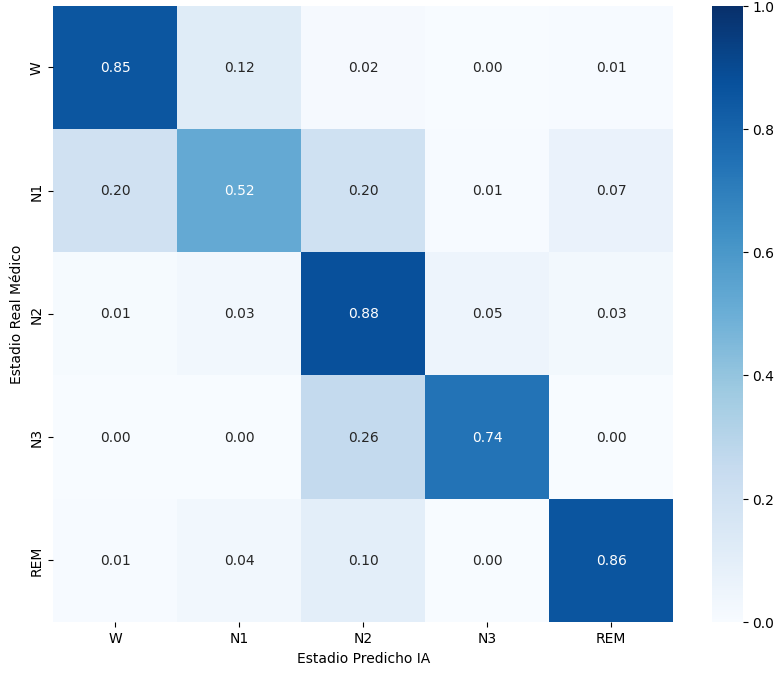
\includegraphics[width=\linewidth]{matriz_v4_interna.png}
        \caption{Validación Interna (V4)}
        \label{fig:matriz_a}
    \end{subfigure}\hfill
    % Panel B: Domain Shift V4 (Hold-Out limpio)
    \begin{subfigure}{0.32\textwidth}
        \centering
        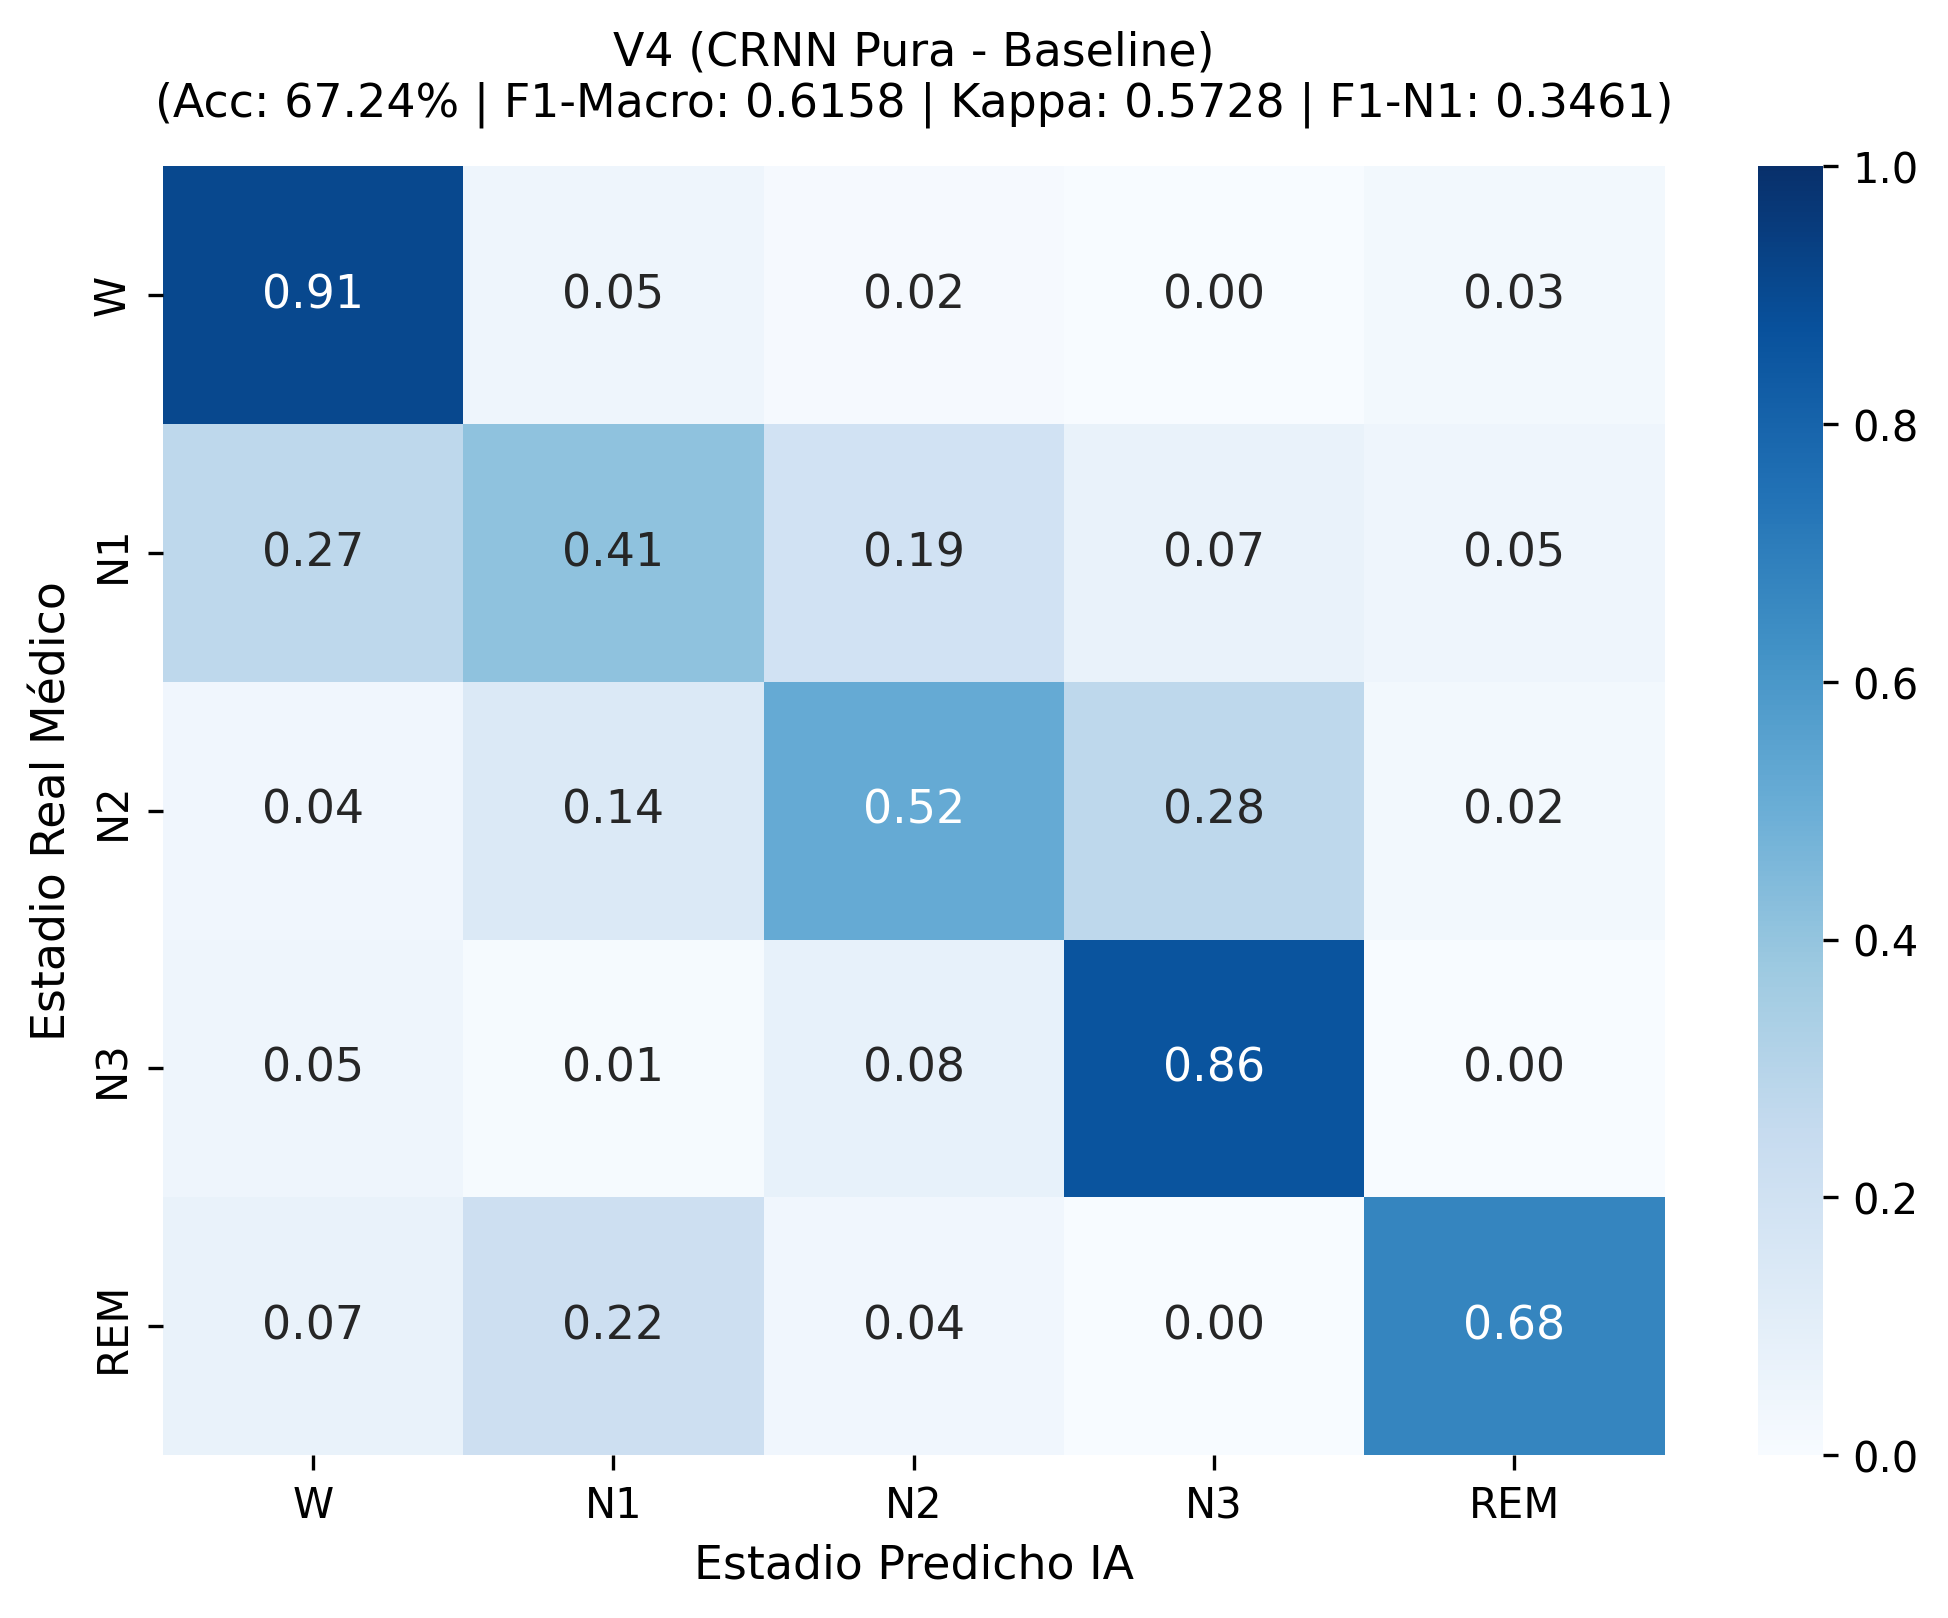
\includegraphics[width=\linewidth]{01_matriz_v4_crnn_pura_baseline.png}
        \caption{Domain Shift en Hold-Out (V4)}
        \label{fig:matriz_b}
    \end{subfigure}\hfill
    % Panel C: Recuperación V7 Exp 4 (Hold-Out limpio)
    \begin{subfigure}{0.32\textwidth}
        \centering
        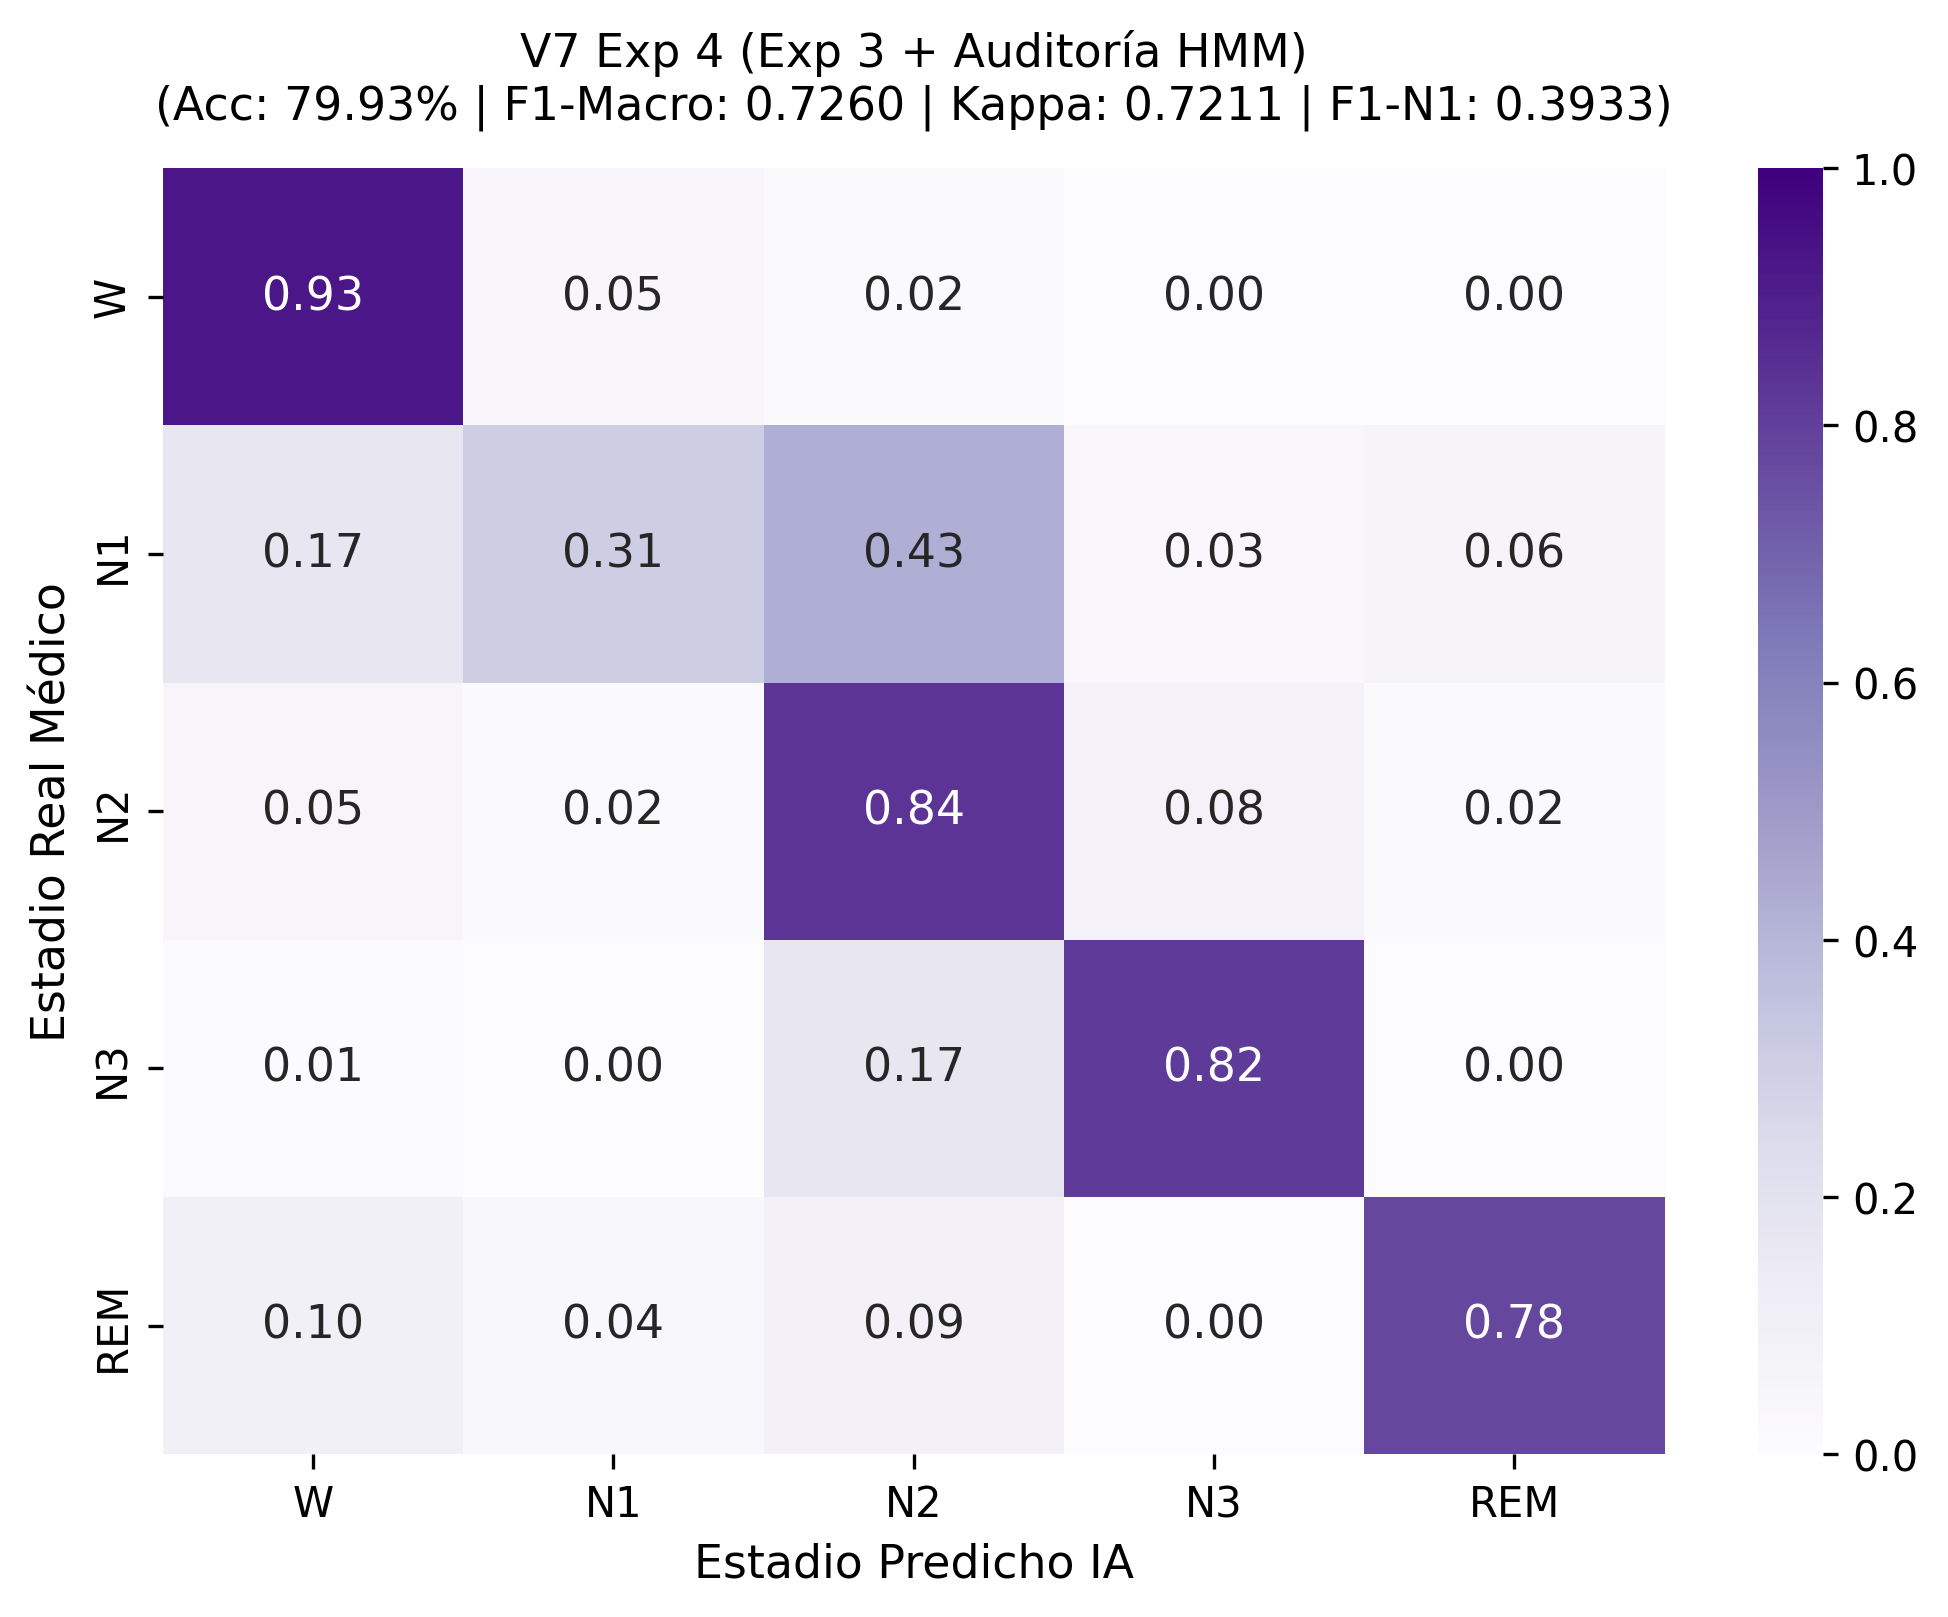
\includegraphics[width=\linewidth]{11_matriz_v7_exp_4.png}
        \caption{Recuperación (V7 Exp 4)}
        \label{fig:matriz_c}
    \end{subfigure}

\caption{Impacto visual del \textit{Domain Shift} y el entrenamiento multicohorte con fusión espectral. (a) La validación interna muestra una alta densidad en la diagonal principal. (b) La CRNN fundacional (V4) se degrada al enfrentarse a la cohorte externa. (c) El porcentaje de aciertos se recupera en varios estadios con la fusión espectral de 528 dimensiones y el HMM de V7.}
\label{fig:matrices_confusion}
\end{figure*}

\subsection{Ablación de V8 en la reserva común}
La receta 59/41 alcanzó 0.7791 de F1 macro frente a 0.7286 del mejor V7 en esta métrica (Exp.~3), una diferencia descriptiva de 5.05 puntos porcentuales. La fusión superó en 2.62 puntos a la CRNN sola (IC del 95\,\% de $+1.79$ a $+3.41$). Frente a DART solo, la diferencia se redujo a $+0.25$ puntos y el intervalo incluyó cero (de $-0.60$ a $+1.22$). La mayor parte del rendimiento global de la fusión ya estaba presente en la rama tabular.

Como contraste adicional, una ejecución previa entrenó V8 sobre las mismas 84 noches y lo comparó con V6 fase C en otras 19 noches de 10 personas de \textit{Cassette} ($26\,653$ épocas emparejadas). V8 obtuvo 0.6855 de F1 macro y V6 obtuvo 0.6432. La diferencia fue de $+4.23$ puntos (IC pareado del 95\,\% de $+1.48$ a $+6.45$). El menor F1 absoluto de ambos modelos muestra cuánto cambia la dificultad con los sujetos evaluados.

\subsection{Sensibilidad por Estadio y Análisis Visual}
El Cuadro \ref{tab:global_metrics} desglosa el F1-Score por clase AASM a lo largo de todas las fases evaluadas en el \textit{Hold-Out} limpio. Desde la línea base V4 hasta V7, los estadios consolidados mostraron recuperaciones claras: N2 pasó de 0.64 a 0.82, N3 de 0.48 a 0.70 y REM de 0.74 a 0.83. En N1, la rama espectral y los pesos de clase (Exp 1 a Exp 3) mantuvieron un F1 de 0.41, mientras que el HMM (Exp 4) mejoró REM (0.83) y el rendimiento global a costa de reducir F1-N1 a 0.39. Visualmente, la Figura \ref{fig:matrices_confusion}(c) confirma la recuperación de la diagonal principal en los estadios consolidados (W, N2, N3 y REM). N1 concentra errores frente a N2 y W.


En V8, la mezcla 59/41 elevó el F1 de N1 a 0.4959. Identificó correctamente $1\,224$ de las $2\,492$ épocas N1 (49.1\,\%) y asignó 820 a N2 (32.9\,\%). La Figura~\ref{fig:confusion_v8} muestra por qué el avance en F1 macro todavía deja sin resolver cerca de la mitad de las épocas N1.

\begin{figure}[tbp]
\centering
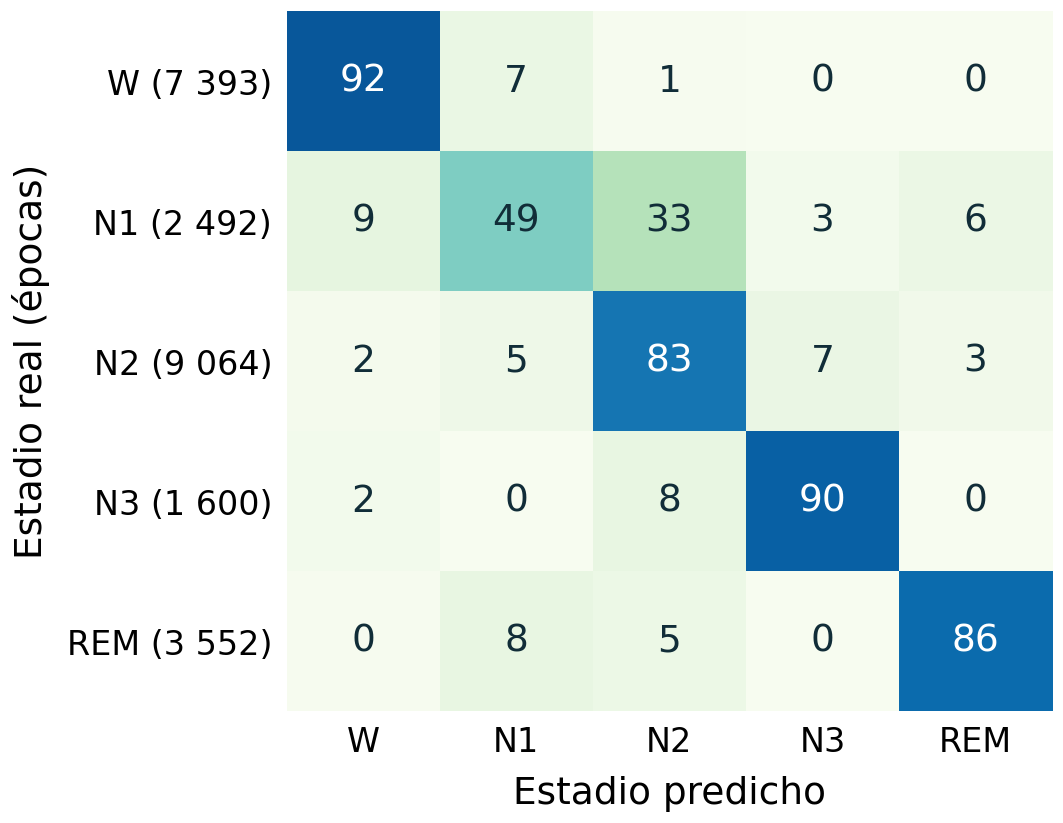
\includegraphics[width=.91\columnwidth]{matriz_v8_fusion.png}
\caption{Fusión V8 (59/41) en la reserva común. Cada fila indica el porcentaje de épocas de un estadio real asignado a cada predicción. Entre paréntesis se indica el soporte.}
\label{fig:confusion_v8}
\end{figure}

\subsection{Contexto frente al Estado del Arte}
El Cuadro~\ref{tab:sota_comparison} contextualiza los resultados en \textit{Sleep-EDF}. Los estudios publicados difieren en la composición de las cohortes, el tratamiento de la vigilia y la estrategia de validación. La comparación directa entre nuestras arquitecturas se basa en las épocas comunes del Cuadro~\ref{tab:global_metrics}.

\begin{table}[htbp]
\centering
\caption{Referencia Contextual frente al Estado del Arte en \textit{Sleep-EDF} (Protocolos No Equivalentes)}
\label{tab:sota_comparison}
\resizebox{\columnwidth}{!}{%
\begin{tabular}{|l|l|c|c|c|}
\hline
\textbf{Modelo / Estudio} & \textbf{Evaluación} & \textbf{Acc.} & \textbf{F1-M} & \textbf{Kappa} \\ \hline
DeepSleepNet \cite{supratak2017} & EDF-20, 20 pliegues & 0.820 & 0.769 & 0.76 \\ \hline
TinySleepNet \cite{supratak2020} & EDF-78, 10 pliegues & 0.831 & 0.781 & 0.77 \\ \hline
AttnSleep \cite{eldele2021} & EDF-78, 20 pliegues & 0.813 & 0.751 & 0.74 \\ \hline
U-Sleep \cite{perslev2021} & SEDF-SC, 23 registros & --- & 0.790 & --- \\ \hline
V7, Exp. 3 & Reserva (20 noches) & 0.797 & 0.729 & 0.72 \\ \hline
V7, Exp. 4 & Reserva (20 noches) & 0.799 & 0.726 & 0.72 \\ \hline
V8, 59/41 & Reserva (20 noches) & 0.831 & 0.779 & 0.77 \\ \hline
\end{tabular}%
}
\end{table}

%===========================================================
\section{Discusión y Limitaciones}
%===========================================================
\textbf{Compromiso del HMM y Sensibilidad en N1:}
En V7, añadir información espectral y contexto nocturno elevó el F1 macro de 0.7139 (V6, 192 dimensiones) a 0.7286 (V7, Exp.~3). Viterbi favoreció la continuidad del hipnograma y mejoró la exactitud global, a costa de reducir el F1 de N1 de 0.4144 a 0.3933. Esto motivó probar una segunda fuente de probabilidades que pudiera intervenir en cada época de transición.

\textbf{Normalización Nocturna y Resiliencia Arquitectónica:}
Ambas arquitecturas aprovechan información posterior a la época clasificada. V7 calcula los estadísticos nocturnos sobre el registro recortado y V8 extrae el contexto de la noche completa antes de puntuar sus épocas elegibles. Su aplicación corresponde a la lectura retrospectiva de la polisomnografía. La tolerancia a un canal auxiliar ausente está implementada en el preprocesamiento. Cuantificar su efecto requiere retirar cada sensor de forma controlada.

\textbf{Limitaciones del Estudio:}
La reserva fija de \textit{Cassette} intervino en decisiones de V4--V7. Aunque los diez sujetos quedaron fuera del nuevo ajuste de V8, en el estudio mixto previo nueve habían contribuido al ajuste y SC429 a la selección de la configuración. SC426 también participó en el estudio tabular inicial. La comparación estima rendimiento retrospectivo. Los intervalos entre ramas de V8 reflejan la variabilidad de diez personas y condicionan sobre un único ajuste. Para V7 se conservaron métricas agregadas, lo que limita la comparación V8--V7 a diferencias descriptivas en esta reserva. La utilidad clínica y la latencia del flujo completo de \textit{SleepAI Studio} requieren validación prospectiva.

%===========================================================
\section{Conclusiones y Trabajo Futuro}
%===========================================================
\subsection{Conclusiones}
En la reserva común, las características espectrales y el contexto nocturno elevaron el F1 macro hasta 0.7286 en V7. V8 retomó los descriptores tabulares explorados en V2 y el contexto espectral nocturno de V7. El cambio fue entrenar cada rama para predecir el estadio y combinar después sus probabilidades. Con el entrenamiento limitado a 43 sujetos, la mezcla 59/41 alcanzó 0.7791 de F1 macro y 0.4959 en N1. Respecto de DART, la fusión mejoró N1 y REM a costa de N3, con incertidumbre en la ganancia global. La siguiente prueba debe conservar las configuraciones fijadas y reservar una cohorte ajena a toda la selección.

\subsection{Trabajo Futuro}
Las siguientes etapas se centrarán en: (1) evaluar el modelo en cohortes externas completamente independientes con patologías severas (ej., SHHS y MESA del NSRR) incorporando intervalos de confianza por \textit{bootstrap}; (2) ejecutar pruebas empíricas de tolerancia a pérdida de canales, latencia de inferencia y calibración de incertidumbre para validar el flujo \textit{Human-in-the-Loop} en \textit{SleepAI Studio}; y (3) explorar los \textit{embeddings} latentes y el hipnograma como biomarcadores predictivos de patologías, en línea con los modelos fundacionales multimodales recientes \cite{thapa2026nature}.

%===========================================================
\section*{Declaraciones}
%===========================================================
\textbf{Disponibilidad de Datos y Ética:} Se utilizaron datos públicos y anonimizados de \textit{Sleep-EDF Database Expanded} alojados en PhysioNet bajo licencia abierta (ODC-By 1.0). \textbf{Conflicto de Intereses y Financiación:} Los autores declaran no tener conflictos de intereses; este trabajo fue desarrollado sin financiación externa en el marco de la Maestría en Inteligencia Artificial de la Universidad de los Andes. \textbf{Contribución de Autores:} Todos los autores contribuyeron equitativamente en la conceptualización, implementación, análisis de resultados y redacción del manuscrito.

\textbf{Reproducibilidad.} El repositorio del proyecto conserva las versiones de datos y recetas con DVC. Los cuadernos \path{DatosV4.ipynb} y \path{experimento_8_holdout_datosv4.ipynb}, en la carpeta \path{Notebooks/experiments}, documentan la selección de noches, las métricas históricas y la ablación de V8. El segundo cuaderno incluye la comparación completa con las variantes exploratorias, algunas con mayor F1 macro en esta reserva. La receta original está en \path{Notebooks/dart_crnn_mixto.ipynb}.

\textbf{Uso de Inteligencia Artificial Generativa:} Durante la preparación de este trabajo, los autores utilizaron Google Gemini y Codex como herramientas de apoyo para la lluvia de ideas sobre refinamientos arquitectónicos, asistencia en la generación y depuración de código en Python, y revisión de estilo y redacción académica. El cuaderno de V8 registra las comprobaciones de partición y las métricas obtenidas. Los autores asumen la responsabilidad por la integridad y exactitud de la publicación.

%===========================================================
\renewcommand{\refname}{Referencias}
\IEEEtriggeratref{14}
\begin{thebibliography}{99}
%===========================================================

\bibitem{berry2020}
R. B. Berry, R. Brooks, C. E. Gamaldo, S. M. Harding, R. M. Lloyd, C. L. Marcus, y B. V. Vaughn, \textit{The AASM Manual for the Scoring of Sleep and Associated Events: Rules, Terminology and Technical Specifications}. Darien, IL, EE. UU.: American Academy of Sleep Medicine, 2020.

\bibitem{kemp2000}
B. Kemp \textit{et al.}, ``Analysis of a sleep-dependent neuronal feedback loop: the slow-wave microcontinuity of the EEG,'' \textit{IEEE Transactions on Biomedical Engineering}, vol. 47, no. 9, pp. 1185--1194, 2000, doi: \url{https://doi.org/10.1109/10.867928}.

\bibitem{supratak2020}
A. Supratak y Y. Guo, ``TinySleepNet: An efficient deep learning model for sleep stage scoring based on raw single-channel EEG,'' en \textit{Proc. 42nd Annu. Int. Conf. IEEE Eng. Med. Biol. Soc. (EMBC)}, 2020, pp. 641--644, doi: \url{https://doi.org/10.1109/EMBC44109.2020.9176741}.

\bibitem{ke2017}
G. Ke \textit{et al.}, ``LightGBM: A highly efficient gradient boosting decision tree,'' en \textit{Advances in Neural Information Processing Systems (NeurIPS)}, vol. 30, 2017.

\bibitem{dart2015}
R. Korlakai Vinayak y R. Gilad-Bachrach, \emph{DART: Dropouts meet Multiple Additive Regression Trees}, en \textit{Proc. 18th Int. Conf. Artificial Intelligence and Statistics}, PMLR, vol. 38, pp. 489--497, 2015. \url{https://proceedings.mlr.press/v38/korlakaivinayak15.html}.

\bibitem{supratak2017}
A. Supratak, H. Dong, C. Wu, y Y. Guo, ``DeepSleepNet: A model for automatic sleep stage scoring based on raw single-channel EEG,'' \textit{IEEE Transactions on Neural Systems and Rehabilitation Engineering}, vol. 25, no. 11, pp. 1998--2008, 2017, doi: \url{https://doi.org/10.1109/TNSRE.2017.2721116}.

\bibitem{perslev2021}
M. Perslev, S. Darkner, L. Kempfner, M. Nikolic, P. J. Jennum, y C. Igel, ``U-Sleep: resilient high-frequency sleep staging,'' \textit{npj Digital Medicine}, vol. 4, no. 1, art. 72, 2021, doi: \url{https://doi.org/10.1038/s41746-021-00440-5}.

\bibitem{phan2023}
H. Phan \textit{et al.}, ``L-SeqSleepNet: Whole-cycle long sequence modeling for automatic sleep staging,'' \textit{IEEE Journal of Biomedical and Health Informatics}, vol. 27, no. 10, pp. 4748--4757, 2023, doi: \url{https://doi.org/10.1109/JBHI.2023.3303197}.

\bibitem{eldele2021}
E. Eldele \textit{et al.}, ``An attention-based deep learning approach for sleep stage classification with single-channel EEG,'' \textit{IEEE Transactions on Neural Systems and Rehabilitation Engineering}, vol. 29, pp. 809--818, 2021, doi: \url{https://doi.org/10.1109/TNSRE.2021.3076234}.

\bibitem{geirhos2020shortcut}
R. Geirhos, J.-H. Jacobsen, C. Michaelis, R. Zemel, W. Brendel, M. Bethge, y F. A. Wichmann, ``Shortcut learning in deep neural networks,'' \textit{Nature Machine Intelligence}, vol. 2, no. 11, pp. 665--673, 2020, doi: \url{https://doi.org/10.1038/s42256-020-00257-z}.

\bibitem{sleepedfx_dataset}
B. Kemp, A. H. Zwinderman, B. Tuk, H. A. Kamphuisen, y J. J. Oberyé, ``Sleep-EDF Database Expanded (version 1.0.0),'' \textit{PhysioNet}, 2018, doi: \url{https://doi.org/10.13026/C2X676}.

\bibitem{goldberger2000}
A. L. Goldberger \textit{et al.}, ``PhysioBank, PhysioToolkit, and PhysioNet: components of a new research resource for complex physiologic signals,'' \textit{Circulation}, vol. 101, no. 23, pp. e215--e220, 2000, doi: \url{https://doi.org/10.1161/01.cir.101.23.e215}.

\bibitem{gramfort2013}
A. Gramfort \textit{et al.}, ``MEG and EEG data analysis with MNE-Python,'' \textit{Frontiers in Neuroscience}, vol. 7, art. 267, 2013, doi: \url{https://doi.org/10.3389/fnins.2013.00267}.

\bibitem{akiba2019optuna}
T. Akiba, S. Sano, T. Yanase, T. Ohta, y M. Koyama, ``Optuna: A next-generation hyperparameter optimization framework,'' en \textit{Proc. 25th ACM SIGKDD Int. Conf. Knowl. Discov. Data Min.}, 2019, pp. 2623--2631, doi: \url{https://doi.org/10.1145/3292500.3330701}.

\bibitem{lin2017}
T.-Y. Lin, P. Goyal, R. Girshick, K. He, y P. Dollár, ``Focal loss for dense object detection,'' en \textit{Proc. IEEE Int. Conf. Comput. Vis. (ICCV)}, 2017, pp. 2980--2988, doi: \url{https://doi.org/10.1109/ICCV.2017.324}.

\bibitem{thapa2026nature}
R. Thapa \textit{et al.}, ``A multimodal sleep foundation model for disease prediction,'' \textit{Nature Medicine}, vol. 32, pp. 752--762, 2026, doi: \url{https://doi.org/10.1038/s41591-025-04133-4}.

\end{thebibliography}

\end{document}
